\documentclass[12pt,a4paper]{article}
\usepackage[T2A]{fontenc}
\usepackage[utf8]{inputenc}
\usepackage[russian]{babel}
\usepackage{amsmath,amssymb,geometry,graphicx,hyperref,longtable,fvextra}
\geometry{margin=18mm}
\hypersetup{hidelinks}
\setlength{\parindent}{0pt}
\setlength{\parskip}{5pt}
\begin{document}
\begin{center}\large Лабораторная работа №2. Метод ломаных\end{center}
Борисюк Е. Г.
\par\textbf{Постановка}\par
Требуется программа для глобального
экстремума липшицевой функции, заданной строкой, на отрезке с точностью $\varepsilon$.
Для демонстрации выбираю одномерное сечение функции Растригина:
\[
R(x,y)=20+x^2+y^2-10\cos(2\pi x)-10\cos(2\pi y),
\]
\[
f(x)=R(x,0)=x^2+10(1-\cos(2\pi x))\to\min,
\quad [a,b]=[-2,2],\quad\varepsilon=0{,}01.
\]
\par\textbf{Локальные минимумы и точный ответ}\par
\[
f'(x)=2x+20\pi\sin(2\pi x),\quad
f''(x)=2+40\pi^2\cos(2\pi x).
\]
На $[3/4,1]$ имеем $f''(x)\ge2>0$, $f'(3/4)<0$ и $f'(1)=2>0$.
Значит, внутри этого интервала есть строгий локальный минимум.
Функция чётная, поэтому симметричный минимум есть и на $[-1,-3/4]$.
Кроме того, $x=0$ --- строгий глобальный минимум:
\[
f(x)\ge x^2\ge0,\qquad f(0)=0.
\]
Таким образом, требование минимум двух локальных минимумов выполнено.
\par\textbf{Константа Липшица}\par
На отрезке $[-2,2]$:
\[
|f'(x)|\le2|x|+20\pi|\sin(2\pi x)|\le4+20\pi.
\]
Выбираю $L=4+20\pi\approx66{,}83185307$. Это допустимая верхняя оценка,
не обязательно наименьшая возможная константа.
\par\textbf{Формулы метода}\par
Из условия Липшица $|f(x)-f(x_i)|\le L|x-x_i|$ следует
\[
f(x)\ge f(x_i)-L|x-x_i|.
\]
Нижняя ломаная $p(x)=\max_i\{f(x_i)-L|x-x_i|\}$ не выше исходной функции.
Для соседних верхних вершин $(x_i,f_i)$ и $(x_{i+1},f_{i+1})$
пересекаю прямые $f_i-L(x-x_i)$ и $f_{i+1}-L(x_{i+1}-x)$:
\[
\boxed{\xi_i=\frac{x_i+x_{i+1}}2-\frac{f_{i+1}-f_i}{2L}},\qquad
\boxed{\eta_i=\frac{f_i+f_{i+1}-L(x_{i+1}-x_i)}2}.
\]
Выбираю наименьшую $\eta_i$, вычисляю $f(\xi_i)$ и заменяю один интервал двумя.
Верхняя оценка $U=\min_i f_i$, нижняя $\ell=\min_i\eta_i$.
Остановка: $U-\ell\le\varepsilon$. Тогда $\ell\le f^*\le U$,
то есть ошибка по значению функции не превосходит $\varepsilon$.
\newpage
\par\textbf{Первые шаги вручную}\par
В концах $f(-2)=f(2)=4$, поэтому $U_0=4$.
Первая нижняя вершина:
\[
\xi_0=0,\qquad \eta_0=4-2L\approx-129{,}66370614.
\]
Вычисляю $f(0)=0$, получаю $U_1=0$. На двух новых интервалах:
\[
\xi_{\text{лев}}=-1+\frac2L\approx-0{,}970074,
\quad \xi_{\text{прав}}=1-\frac2L\approx0{,}970074,
\quad\eta=2-L\approx-64{,}83185307.
\]
При равенстве нижних оценок программа выбирает левый интервал.
Хотя точный минимум уже найден, остановиться нельзя: пока нижняя оценка
не исключает более глубокие минимумы в других частях отрезка.
Алгоритм продолжает уточнять ломаную до требуемого разрыва.
\begin{center}\small
\begin{tabular}{r|r|r|r|r}
Новых проб & Следующая точка $\xi$ & $U$ & $\ell$ & $U-\ell$\\\hline
0 & 0.000000 & 4.000000 & -129.663706 & 133.663706\\
1 & -0.970074 & 0.000000 & -64.831853 & 64.831853\\
2 & 0.970074 & 0.000000 & -64.831853 & 64.831853\\
3 & -1.463470 & 0.000000 & -31.857277 & 31.857277\\
4 & -0.476678 & 0.000000 & -31.857277 & 31.857277\\
5 & 0.476678 & 0.000000 & -31.857277 & 31.857277\\
\end{tabular}\end{center}
\par\textbf{Результат вычислений}\par
Новых проб: 131; вычислений функции вместе с концами: 133.
\[\ell=-0.00862795,\quad U=0.00000000,\quad U-\ell=0.00862795\le0{,}01.\]
\[
\boxed{x_{\min}\approx0,\qquad f(x_{\min})\approx0.}
\]
Независимая проверка: $f(x)\ge0$ и $f(0)=0$.
Точность в условии остановки относится к значению функции.
\newpage
\par\textbf{Основная программа на Kotlin/JVM}\par
Метод ломаных реализован на Kotlin. Готовые оптимизаторы не используются.
На вход передаются строка функции, границы $a,b$ и точность $\varepsilon$.
Дополнительно можно указать направление экстремума и известную константу $L$.
Для максимума минимизируется $-f(x)$ с восстановлением исходных границ.

Основные части программы:
\begin{itemize}
\item \texttt{ExpressionParser}, \texttt{evaluate} --- разбор строки и вычисление функции;
\item \texttt{expressionBound} --- аналитическая верхняя оценка $L$;
\item \texttt{intersection} --- пересечение опорных прямых;
\item \texttt{piyavskii} --- выбор интервала, новая проба и остановка;
\item \texttt{plotResult} --- исходная функция и итоговая ломаная в PNG.
\end{itemize}
Верхние вершины хранятся в \texttt{TreeMap}, нижние вершины интервалов ---
в \texttt{PriorityQueue}. После одной пробы выбранный интервал заменяется
двумя. Поиска минимума по равномерной сетке нет: точки сетки создаются только
при рисовании. График строится средствами Java2D, без сторонних библиотек.

Автоматическая оценка $L$ получается по структуре выражения. Если оценку
получить не удалось, требуется корректная константа пользователя.
Проверка уже известных секущих может выявить неверное $L$, но не доказывает
его корректность на всём отрезке.
\par\textbf{Запуск основной версии}\par
Готовый JAR включает стандартную библиотеку Kotlin; для запуска нужна Java 17+:
\begin{Verbatim}[fontsize=\small,breaklines=true]
java -jar kotlin/lab02.jar
java -jar kotlin/lab02.jar "(x-0.37)**2" -1 2 0.01
\end{Verbatim}
Исходник: \texttt{kotlin/src/main/kotlin/Main.kt}.\par
Для сборки предусмотрены Gradle-конфигурация и скрипт \texttt{kotlin/build.ps1}.
\par\textbf{Дополнительная версия в Google Colab}\par
Основная реализация выполнена на Kotlin. Дополнительная Python-версия для
Google Colab подготовлена с помощью ИИ-генерации: Kotlin-код переписан на
Python с сохранением алгоритма. После перевода проверены разбор выражений,
формулы пересечений, выбор интервалов, критерий остановки и итоговый ответ.
Эта версия сохранена на случай необходимости запуска в браузере.

Обе реализации проверены на смещённой параболе, линейной и постоянной
функциях, модуле и задаче на максимум. На Растригине результаты совпали:
$x=0$, $f(x)=0$, 131 итерация, 133 вычисления, разрыв $0{,}0086279513$.
Время локальных запусков: Kotlin --- 0.004278 с, Python --- 0.000501 с.
Измеряется сам алгоритм, без разбора выражения и построения графика;
время зависит от среды и может отличаться при повторном запуске.
\newpage
\par\textbf{Визуализация результата}\par
График получен основной Kotlin-программой. Слева показаны исходная функция, итоговая нижняя ломаная, вычисленные точки
и найденный минимум. Справа --- увеличение около минимума.
\begin{center}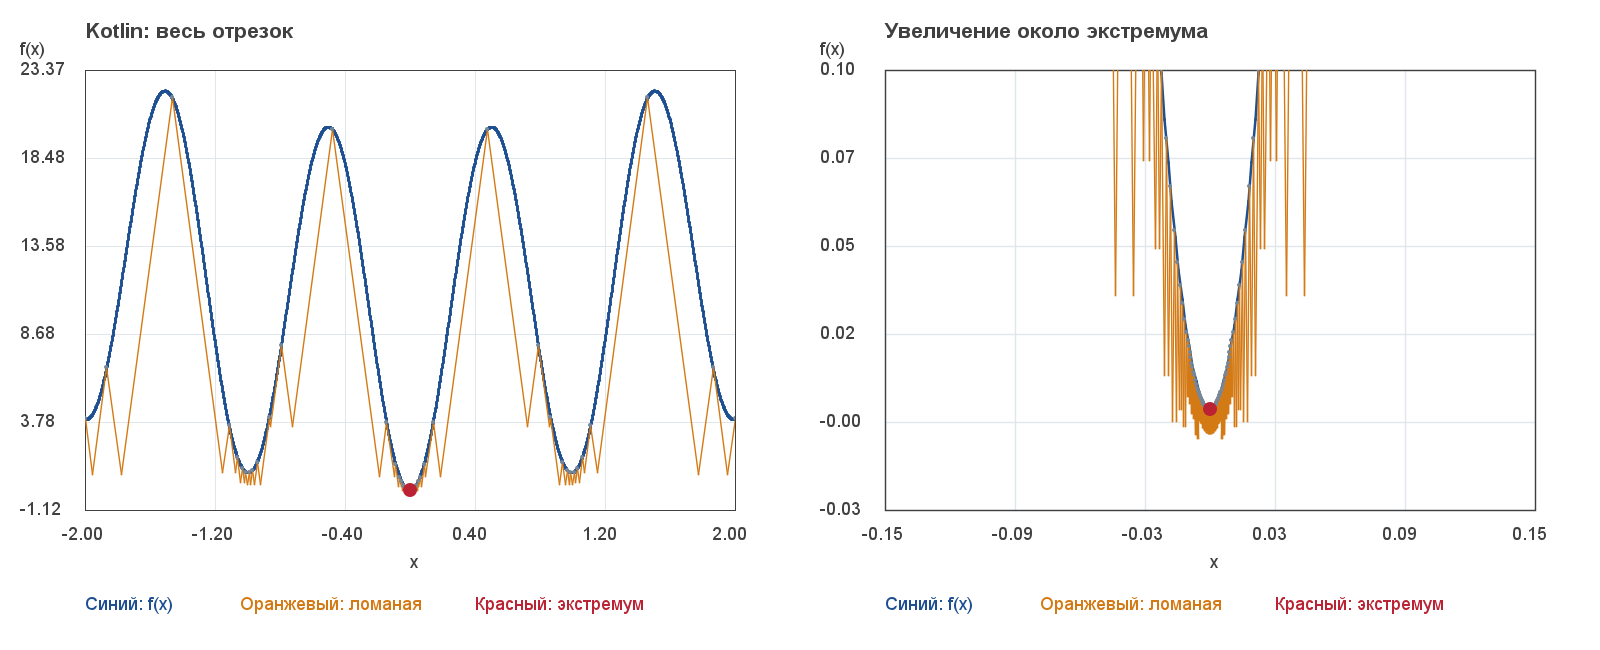
\includegraphics[width=\linewidth]{kotlin-visualization.png}\end{center}
\[
\boxed{x_{\min}\approx0,\qquad f_{\min}\approx0.}
\]
\par\textbf{Ссылки и файлы}\par
\href{https://colab.research.google.com/drive/1tGa_qdx4pisK6OJUMDYsK57pUUTB7RtJ}{Дополнительная Python-версия в Google Colab}.\par
\href{https://github.com/Doney888/methods-of-optimization/tree/main/lab-02}{Материалы лабораторной в GitHub}: исходное задание.\par
\texttt{kotlin/} --- основной код и готовый JAR.\par
\texttt{python-solution.ipynb}, \texttt{piyavskii.py} --- дополнительный перевод.\par
\texttt{kotlin-visualization.png}, \texttt{report.pdf}, \texttt{report.tex}.
\par\textbf{Рефлективный вывод}\par
Я разобрал, как условие Липшица позволяет оценивать функцию снизу и искать
глобальный минимум среди нескольких локальных. Основной трудностью было
различить найденное хорошее значение и доказанную точность: даже после
попадания в $x=0$ нужно уточнять нижнюю ломаную. Для проверки использовал
известный аналитический минимум и контролировал разрыв оценок. Основной код
оформил на Kotlin; дополнительную Python-версию получил с помощью ИИ-перевода
и проверил совпадение результатов.
\end{document}